\documentclass[a4paper,12pt]{scrreprt}

\usepackage{german}
\usepackage{graphicx}
\usepackage{rotating}

\title{Sudoku3D}
\subtitle{Projekt 3. Lehrjahr MTS51}
\author{Niclas Hofmann, Son Le Cong \& Marvin Mahn}
\date{1. Juni 2018}


\begin{document}
	\maketitle
	\tableofcontents
	
	\chapter{Einf\"uhrung}
	\section{Vorwort}
	Die vorliegende Dokumentation wurde von den Autoren im Rahmen des Projektes im dritten Lehrjahres
	f\"ur das Lernfeld 13 erstellt.\medskip \\
	Zur Unterscheidung, welche Texte von welchen Autoren verfa{\ss}t wurden, wird dies an den jeweiligen
	Stellen erw\"ahnt\footnote{Ist kein Name angef\"uhrt war der Autor Niclas Hofmann}.
	Sinnvollerweise beschreibt jeder Autor die von ihm erstellten Teile des Projektes.
	
	\section{Problemdefinition}
	Herk\"ommliche Sudokus k\"onnen je nach Schwierigkeitsgrad zwar an Komplexit\"at gewinnen,
	bleiben aber dennoch recht schnell l\"osbar. Auch Sonderformen wie Killer-Sudokus\footnote{
	https://de.wikipedia.org/wiki/Killer-Sudoku} oder X-Sudokus\footnote{https://de.wikipedia.org/
	wiki/Sudoku\#X-Sudoku} bieten nur bis zu einem gewissen Grad weiteren Anreiz.

	\section{Projektziel}
	Um etwas neuartiges zu schaffen, das genau diesen Anreiz bietet, soll nun ein Programm erstellt
	werden, welches 3D-Sudokus kreiert, analog zum 3D-Schach aus der Fernsehserie Star Trek.
	\medskip \\
	Aber auch hier soll es m\"oglich sein, nicht nur mit den Standardregeln zu spielen, sondern auch
	andere verwenden zu k\"onnen.\medskip \\
	Au{\ss}erdem soll das Endprodukt als interaktives Spiel auf der MATSE-Hompage\footnote{
	https://www.matse-ausbildung.de/} angeboten werden.

	\section{Wichtige Termine}
	Diese Projekt mu{\ss} am 1. Juni 2018 pr\"asentiert werden.
	
	\chapter{Entwicklerdokumentation}
	\section{Model}
	\subsection{Problemanalyse}
	F\"ur das Model fallen die folgenden Aufgaben an:
	\begin{enumerate}
		\item Erstellung eines Sudoku3D's nach den ausgew\"ahlten Regelmodulen
		\item Entfernung einiger Zahlen, um ein spielbares Sudoku3D anzubieten
		\item Speicherung der Daten (vorgegebene Zahlen und User-Eingaben)
		\item \"Uberpr\"ufung, ob das Sudoku3D gel\"ost wurde
		\item Ein $clear$, das alle User-Eingaben entfernt
		\item Die Zur\"uckgabe aller falsch eingetragenen zahlen
		\item Wiederherstellung eines Sudoku3D's mit gegebenen Zahlen, Regelmodulen und
			User-Eingaben
	\end{enumerate}

	\subsubsection{Regelmodule}
	Da zum Erstellen eines Sudoku3D's Regelmodule ben\"otigt werden, m\"u{\ss}en diese vorhanden
	sein. Doch was ist/leistet ein Regelmodul?\medskip \\
	Ein Regelmodul definiert alle Einheiten (Units), in denen die Zahlen von 1-9 nur einmal vorkommen
	d\"urfen. Bei einem normalen Sudoku sind dies z. B. die 3x3 Boxen, die Zeilen und die Spalten.
	Weil die Unterscheidung zwischen Zeile und Spalte in der Dimension liegt, werden diese im
	Sudoku3D nicht unterschieden. Somit sind die zwei Grundlegenden Regelmodule auch schon
	vorgegeben.

	\section{Controller: Die Schnittstelle (Marvin Mahn)}
	\subsection{Bestandteile}
	Die Schnittstelle soll die Kommunikation zwischen Grafikoberfl\"ache (Client) und den
	Sudokufunktionen (Server) erm\"oglichen.\medskip \\
	Zuerst stand die Idee einen Applikationsserver selbst hierf\"ur zu kreieren. Jedoch lies ein
	erster Fehlschlag eines Prototypen diese Idee zerplatzen, weshalb der Fokus vorerst auf fertige
	Server fiel. Vorteilhaft dabei ist, da{\ss} es mit Java EE eine f\"ur dieses Projekt bereits
	ausreichend vorgegebene Leitfaden gibt. Es stehen zudem eine Vielzahl von kostenlosen
	Applikationsservern zu Verf\"ugung, auf denen wir unsere Applikation ohne gr\"o{\ss}ere
	Schwierigkeiten aufsetzen k\"onnen. Diese Server haben von Hause aus M\"oglichkeiten wie
	Logging, Datenbankanbindung, Diensteinrichtung, etc., um die wir uns nicht mehr sorgen
	m\"u{\ss}en und folglich uns erlauben, alle Aufmerksamkeit der Oberfl\"ache und der Funktion
	des Spiels zu widmen.\medskip \\
	An dieser Stelle sei gesagt, da{\ss} die Rede von einem Testserver ist. Wie bereits erw\"ahnt soll
	das eigentliche Programm sp\"ater auf einem Apache-Server der MATSE-Webseite laufen. Zu der
	Vielzahl von Servern haben es in die engere Auswahl der Standardserver von Oracle GlassFish,
	die Serverapplikation von JBoss\footnote{inzwischen unter Entwicklung von Red Hat} der
	Wildfly-Server und Apache Tomcat mit dem Tomcat 9 geschafft.\medskip \\
	Die Wahl fiel auf Tomcat 9, da dieser dem MATSE-Server \"anlicher ist. Erst im sp\"ateren Verlauf
	wechselte die endg\"ultige Festlegung auf Tomcat 7,da dies die Tomcat Version ist, die auf dem
	MATSE-Server l\"auft.\medskip \\
	Die Umgebungsspezifikationen sind in folgender Grafik zusammengefa{\ss}t:
	\begin{figure}[h]
		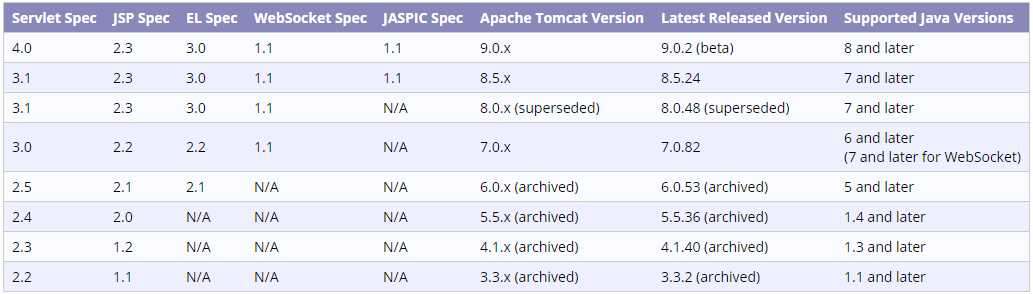
\includegraphics[scale=0.55]{pictures/Tomcat-Versionsvergleich}
		\caption{http://tomcat.apache.org/whichversion.html}
	\end{figure}\\
	Ein weiterer Aspekt des Pakets ist die Einrichtung des Servers und des Spiels, soda{\ss} man nur
	einen Knopf dr\"ucken mu{\ss} um die Anwendung verwenden zu k\"onnen\footnote{Dies entspricht
	einem Installer}. Dieser Teil ist vorerst nicht weiter verfolgt worden. Die Klassen für das Spiel befinden
	sich in einem $WAR$-Archiv. Dieses $WAR$-Archiv wird im Tomcat-Server-Verzeichnis unter $webapps$
	abgelegt. Zu jeder Webapplikation, die \"uber den einen Tomcat-Server l\"auft, wird auch ein Eintrag
	in der $web.xml$, des Servers ben\"otigt. Diese befindet sich im Tomcat-Server-Verzeichnis im Ordner
	$conf$. Beide Installationsvorgaben werden manuell durchgef\"uhrt. F\"ur die Verwendung des
	Serverdashboards des Tomcat-Servers \"uber die Browseroberfl\"ache mu{\ss} eine Administratorrolle
	f\"ur den Server definiert werden. Diese Einstellung erfolgt \"uber die $tomcat$-$users$
	Konfigurationsdatei, im $conf$ Ordner des Tomcat-Server-Verzeichnisses.\medskip \\
	Ist der Server eingerichtet, kann dieser nun Anfragen - in unserem Fall von HTTP-Natur - entgegen
	nehmen. Mit dem Datenmanagement sei ein weiterer und der wichtigste Punkt des Pakets benannt.
	Wie erfolgt die Kommunikation zwischen Client und Server? Nach welchem Aufbau findet das
	\"Ubermitteln von Daten zwischen Client und Server statt? Wie wird das Sudoku einerseits auf
	Clientseite und andererseits auf Serverseite gehalten?

	\subsection{Umsetzung}
	Die Kommunikation erfolgt \"uber HTTP-Anfragen, von Clientseite aus zum Server.
	Die Anfragen selbst erfolgen \"uber die JavaScript-Oberfl\"ache. Da  f\"ur die grafische Oberfl\"ache
	bereits JQuery eingerichtet ist, bedienen wir uns dessen, um mit der \$.ajax-Methode, unkompliziert
	Anfragen an den Server zu stellen. Der $dataType$ der ajax-Request wurde f\"ur diesen Zwecke auf
	JSON (JavaScript Object Notation) festgelegt, da dieser eine direkte Weiterverarbeitung in JavaScript
	erm\"oglicht. Ist nun die Anfrage auf Serverseite angekommen, startet  die Abarbeitung im Servlet.
	Das gute an dem bereits fertigen Server ist dabei, da{\ss} die Threadverteilung intern vom Server
	geregelt wird. So startet jede Anfrage einen neuen Thread, der das Servlet mit der Anfrage ausführt.
	Dies erm\"oglicht asynchrone und f\"ur unseren Fall schnellere Abarbeitung von verschiedenen Funktionen
	der Oberfl\"ache. Es gilt aber auch hier Nachteile der Asynchronit\"at zu beachten, gerade auf
	JavaScript-Seite. Abgesehen vom zeitversetzten Eintreffen der Antworten kann der Server schnell
	lahmgelegt werden, wenn w\"ahrend des Wartens auf eine Antwort die erneute Anfrage, der gleichen
	Funktion nicht blockiert oder anderweitig unterbunden wird.\medskip \\
	Zurück zum Servlet. Das Servlet verarbeitet ausschließlich ihm bekannte Anfragen. F\"ur diesen
	Zweck wird in jeder Anfrage ein Parameter $wahl$ gesetzt, der entsprechend einen String enth\"ahlt.
	Das Servlet leitet die Anfrage weiter an die Klasse $Request\_Bridge$. Diese Klasse f\"uhrt je nach
	Wert die $doWork$ einer der Anfragewahl zugewiesen Request Handler aus. Request Handler
	implementieren die Methode $doWork$ vom Interface $IRequest\_Handler$. Diese Methode liefert in
	allen F\"allen ein JSON-Objekt zur\"uck, da{\ss} das Ergebnis des Handlers enth\"alt. Alle
	Request-Klassen\footnote{au{\ss}er $Request\_Bridge$} erweitern die abstrakte Klasse $AbstractRequest$.
	Diese bietet Unterst\"utzungsmethoden zum Auslesen von Parametern aus einer HTTP-Anfrage.
	Die Handler arbeiten als einzige mit den Sudoku-Klassen und Methoden zusammen.
%	\medskip \\
%	Des Weiteren mu{\ss} die Gr\"o{\ss}e von Sudokus und die Auswahl der Regeln beachtet werden.
%	Da Sudokus aus Kombinationen von Regeln in gewissen Gr\"o{\ss}enordnungen, vom Server nicht schnell
%	genug erzeugt werden konnten (bzw. zu keinem Ergebnis f\"uhrten). Ein erster Test f\"ur ein Sudoku
%	mit Ber\"ucksichtigung von Diagonalen, wurde nach acht Tagen Rechenzeit, ohne Ergebnis abgebrochen.
%	Dies hatte auch zur Folge, dass von den eigentlich gewollten Regeln, ein gro{\ss}er Teil ausgebaut
%	werden mu{\ss}te oder gar nicht erst umgesetzt wurde. Die restlichen Regeln sind f\"ur das Endprodukt
%	nicht vorgesehen.
	\begin{sidewaysfigure}[p]
		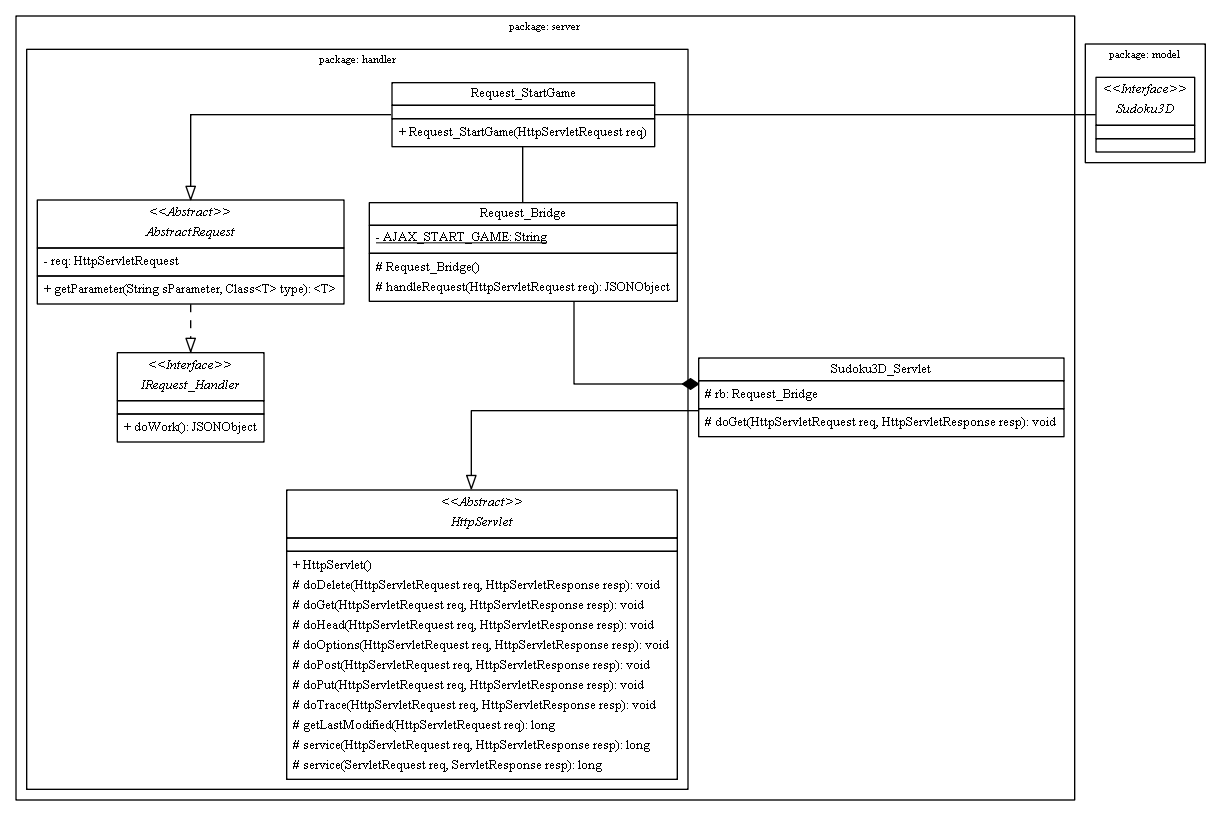
\includegraphics[scale=0.55]{pictures/controller}
		\caption{Server-Paket als UML-Diagramm}
	\end{sidewaysfigure}\medskip \\

	\subsection{Client}
	Client ist jeder Rechner, der mit dem Server kommuniziert. Auf Clientseite wird die Oberfl\"ache des
	Spiels geladen. Zur Oberfl\"ache des Spiels geh\"oren ein Start-Button, ein Neustart-Button zum
	Laden eines neuen Spiels, ein L\"osen-Button zum automatischen L\"osen des Sudokus und ein
	Undo-Button zum Zur\"ucknehmen der letzten Aktion.\medskip \\
	Beim Client werden alle relevanten Daten f\"ur das Spiel gehalten. Dies ermöglicht, nach dem
	Erhalten der Daten vom Server, ein komplettes Offline-Spielen. Sollte das Spiel neugestartet werden,
	wird wieder eine Verbindung zum Server ben\"otigt.

	\subsection{Datenhaltung}
	F\"ur die Datenhaltung in JavaScript ist ein Objekt vorgesehen. Das JSON-Datenformat, da{\ss} von
	Serverseite zur\"uckkommt, ist dabei essentiell. JSON-Objekte in Java erlauben das direkte
	Verarbeiten bzw. Speichern des Sudokus auf Clientseite. Die Daten, die der Server beim Starten des
	Spiels zur\"ucksendet, enthalten die f\"ur den Benutzer sichtbaren Zahlen und die Komplettl\"osung
	des Spiels. Die Komplettl\"osung wird global in das $window$-Attribut des Browsers hinterlegt,
	w\"ahrend die f\"ur den Benutzer sichtbaren Daten in die Felder geladen werden. Die Verbindung
	zum Server wird ausschließlich f\"ur das Erstellen des Spiels gebraucht. Das bietet auch den Vorteil,
	da{\ss} aller Aufwand des Servers allein dem Erstellen der Sudoku-Spiele gewidmet ist. Der Server
	speichert keine Daten. Des Weiteren ist die Funktion des Servers damit auf eine Aufgabe minimiert,
	was m\"ogliche Angriffsflächen verringert.

	\subsection{Speichern und Laden eines Spiels}
	F\"ur das Speichern des Spiels wird lokaler Speicher verwendet. Bei lokalem Speicher handelt es
	sich um eine Speicherform, die in HTML5 als $Web Storage$ spezifiziert ist. Bei dieser Form des
	Speicherns werden Daten lokal im Browser des Clients gespeichert bzw. geladen. Daten aus dem
	lokalen Speicher, k\"onnen ausschlie{\ss}lich \"uber JavaScript oder durch das Leeren des
	Browser-Caches gel\"oscht werden. Das Datenvolumen des Spiels wird durch das 5 MB Speicherlimit
	von $localStorage$ begrenzt. Zu den zu speichernden Daten geh\"ohren der Benutzerstand des Spiels,
	sowie die Komplettl\"osung und die Gr\"o{\ss}e des Sudokus. F\"ur das Spiel ist momentan nur ein
	Speicherslot vorgesehen. Dieser wird automatisch durch das Speichern \"uberschrieben.\medskip \\
	Wird ein Spiel geladen, werden vorher gespeicherte Daten aus dem lokalen Speicher geholt. Der danach
	folgende Aufbau erfolgt wie bei einem Start des Spiels. F\"ur die Ladefunktion wird keine Verbindung
	zum Server ben\"otigt. Sollte der Speicher leer sein, wird eine entsprechende R\"uckmeldung angezeigt.

	\chapter{Benutzerhandbuch}
	\section{Systemvorraussetzungen (Marvin Mahn)}
	Empfohlen wird einer der folgenden Browser:
	\begin{itemize}
		\item Chrome: ab Version 56.0
		\item Internet Explorer: ab Version 11
%		\item Microsoft Edge: ab Version 38.14393
		\item Morzilla Firefox: ab Version 35.0
		\item Safari: ab Version 10.0
		\item Opera: ab Version 11.60
	\end{itemize}

	\section{Benutzerhandbuch (Marvin Mahn)}
	\begin{description}
		\item[Spiel starten] Zum Starten des Spiels mu{\ss} der Start-Button bet\"atigt werden. Das Laden
			des Spiels kann je nach Antwortgeschwindigkeit des Servers und Geschwindigkeit des Browsers
			variieren.
		\item[Spiel neustarten] Zum Neustarten des Spiels, gibt es einen Neustart-Button. Dieser wird
			erst angezeigt, wenn ein Spiel gestartet wurde. Wird der Neustart-Button bet\"atigt, wird ein
			neues Spiel gestartet. Alle vorherigen Spielst\"ande gehen dabei verloren\footnote{Speicherst\"ande
			ausgeschlossen}.
		\item[Spiel speichern] Das Spiel kann \"uber den Speichern-Button gespeichert werden\footnote{
				Vorsicht: Es gibt nur einen Speicherstand! Beim erneuten Speichern wird der alte Stand
				\"uberschrieben}.
		\item[Spiel laden] \"Uber den Laden-Button kann ein gespeicherter Spielstand wiederhergestellt
			werden. Das Spiel wird f\"ur das Laden neu aufgebaut, was l\"angere Zeit in Anspruch nehmen.
		\item[Undo] Mit einem Klick auf den Undo-Button, wird die letzte Aktion r\"uckg\"angig gemacht.
			Dies funktioniert nur einmal bei jeder neuen Aktion.
		\item[Spiel l\"osen] Es wird die L\"osung des Sudoku3Ds eingef\"ugt. Das Spiel gilt dann als beendet.
	\end{description}

	\chapter{Schlu{\ss}wort}
	\section{Fazit}
	\subsection{Controller (Marvin Mahn)}
	Die Zusammenarbeit in einer Gruppe f\"ur ein Projekt, war f\"ur mich eine der gr\"o{\ss}ten
	Herausforderungen.Dabei liegt es weniger an den Personen als eher an der Koordination. Zwar
	hatten wir alle eine \"Ubersicht von dem, was sie machen und zu erledigen haben. Doch die
	unterschiedlichen Arbeitsgeschwindigkeiten und die Aufspaltung der einzelnen Teile war nicht
	leicht zu kombinieren. Ohne $Git$, w\"are eine \"Ubersicht des Fortschritts der Gruppe vermutlich
	wesentlich schwieriger zu verwalten gewesen. Das Zusammenf\"uhren des Quelltextes h\"atte
	deutlich mehr Zeit gekostet und h\"atte vermutlich sonstige Effekte hervorgerufen. Die Controller-
	und Modelseite war dabei das geringste Problem, da diese beiden Seiten keine \"Uberschneidungen
	hatten. Aber die Oberfl\"ache war am schwersten zu verwalten, da sehr schnell \"Uberschneidungen
	im Quelltext vorkamen, die Effekte und Inkonsistenz zur Folge hatten. Son und ich mussten dabei
	mehrfach R\"ucksprache halten, was nicht immer so leicht war. Das Projekt war eine sehr gute
	Erfahrung in punkto Zusammenarbeit. Durch das Austauschen untereinander und die getrennten
	Arbeitsgebiete, kam das Entwicklungsverhalten auch sehr nah an das eines Betriebs in der offenen
	Wirtschaft.

	\section{Ausblick}
	\subsection{Controller (Marvin Mahn)}
	Die Spiel kann auf jeden Fall in seinen Funktionen erweitert werden. Beispielsweise kann neben der
	Undo-Funktion eine Art Redo-Funktion erstellt werden. F\"ur den Benutzer kann auch eine
	Hilfsfunktion eingerichtet werden, die beispielsweise einzelne Zahlen des Ergebnisses verraten kann.
	\medskip \\Die Kommunikation sollte so erweitert werden, da{\ss} HTTPS-Anfragen verwendet
	werden k\"onnen.\medskip \\
	Um Last von dem Benutzer zunehmen, k\"onnte der Server um eine Datenbankanbindung erweitert
	werden, soda{\ss} beim Benutzer nur noch die Benutzer-ID gespeichert wird und der Rest in der
	Datenbank landet. In diesem Zuge sollte dann aber auch der Server besser abgesichert werden. F\"ur
	den Server, samt Webapplikation sollte ein Installer erzeugt werden. Das manuelle Einrichten, ist zwar
	nicht aufwendig, aber kostet dennoch Zeit.
\end{document}
